\documentclass[a4paper,fleqn]{cas-sc}
\usepackage[numbers,sort&compress]{natbib}
\usepackage{amsmath,amssymb,amsthm}
\usepackage{booktabs,array,longtable}
\usepackage{enumitem}
\usepackage{algorithm2e}
\SetKwInput{KwIn}{Input}
\SetKwInput{KwOut}{Output}
\SetKw{KwBreak}{break}
\SetKw{KwRet}{return}
\newlength{\TableWidth}
\theoremstyle{definition}
\newtheorem{definition}{Definition}
\theoremstyle{plain}
\newtheorem{proposition}{Proposition}
\newtheorem{corollary}{Corollary}

\begin{document}
\let\WriteBookmarks\relax
\def\floatpagepagefraction{1}
\def\textpagefraction{.001}
\shorttitle{GB-LCSS for graph-free node classification}
\shortauthors{S. Cao et al.}
\title[mode = title]{Granular ball local consensus for graph-free node classification under label noise}
\author[1]{Silei Cao}
\author[1]{Kun Wang}
\author[2]{Jingyu Zhu}
\author[3]{Tianxing Wang}
\author[1]{Bing Huang}
\cormark[1]
\ead{huangbing@nau.edu.cn}
\affiliation[1]{organization={School of Computer Science, Nanjing Audit University},city={Nanjing},postcode={211815},country={PR China}}
\affiliation[2]{organization={School of Statistics and Data Science, Nanjing Audit University},city={Nanjing},postcode={211815},country={PR China}}
\affiliation[3]{organization={School of Business, Nanjing Audit University},city={Nanjing},postcode={211815},country={PR China}}
\cortext[1]{Corresponding author.}
\begin{abstract}
Graph-free node classification enables prediction from node attributes when graph relations are unavailable or costly to access at deployment. However, existing noise-robust graph methods generally retain graph-dependent inference, whereas graph-free methods have largely been studied with clean training labels. To address this gap, we propose Granular Ball Local-Consensus Soft Supervision (GB-LCSS) for transductive node classification with noisy labels and graph-free inference. GB-LCSS learns node representations through label-free graph contrastive learning, freezes them, and recursively groups nodes into granular balls. For each training node, the observed labels of the other training nodes in its ball form a leave-one-out consensus. A weight determined by their agreement blends this consensus with the node's observed label to produce a soft target for a multilayer perceptron (MLP). This design decouples region construction from noisy-label aggregation and uses local evidence to reduce the influence of isolated annotation errors. Across five datasets and five noise settings, GB-LCSS achieves the highest five-seed mean accuracy in 24 of the 25 settings, compared with seven noisy-label baselines that use the same deployed MLP architecture. Its soft targets also have lower mean Brier scores than the observed one-hot labels in all 25 settings.
\end{abstract}

\begin{highlights}
\item Construct granular balls from graph contrastive representations without labels.
\item Convert training-time graph structure into soft targets for an attribute-only MLP.
\item Refine noisy supervision using leave-one-out consensus within granular balls.
\item Achieve the highest mean accuracy in 24 of 25 settings with the same MLP.
\end{highlights}

\begin{keywords}
label noise \sep node classification \sep graph-free inference \sep graph contrastive learning \sep granular ball computing \sep soft labels
\end{keywords}
\maketitle
\section{Introduction}\label{sec:1}

Node classification is a fundamental task in graph learning, in which node attributes and relationships jointly support prediction. Graph neural networks (GNNs) combine these two sources of information by aggregating representations from neighboring nodes \cite{ref1}. This dependence on graph structure, however, complicates deployment: each prediction requires access to the relevant neighborhood, and retrieving and aggregating multi-hop neighbor information adds computational cost. In applications with missing relations, privacy restrictions, or low-latency requirements, such access may be unavailable or impractical. These constraints have motivated graph-free node classification, in which graph structure is used during training but the deployed classifier receives only node attributes. Graph-MLP \cite{ref3} and GLNN \cite{ref4} demonstrated this approach, and later work such as SimMLP \cite{ref41} and FF-G2M \cite{ref45} refined what structural knowledge is transferred to the multilayer perceptron (MLP) and how. These methods have been developed and evaluated with clean training labels.

In practice, however, training labels obtained through manual annotation, automated rules, or multiple sources may contain errors, and deep models can fit such corrupted annotations \cite{ref24}. On graphs, message passing may propagate the influence of mislabeled nodes to their neighbors \cite{ref6}. Noise-robust graph methods use topology to augment supervision \cite{ref7}, regulate training with noisy labels \cite{ref8}, or select reliable samples \cite{ref9}, but they retain graph access at inference. Graph-free classifiers face a related challenge: errors in the labels used to train an MLP or its teacher can carry over to the deployed model. We study how the training graph can improve noisy-label supervision for a classifier that uses only node attributes at inference.

One way to address this challenge is to combine an observed label with evidence from nearby training nodes. When their labels provide consistent evidence for the underlying class, aggregating them can reduce the influence of isolated annotation errors. Related methods use neighborhood consistency to identify potentially mislabeled samples or encourage agreement between neighboring predictions \cite{ref10,ref11}. For graph data, a graph contrastive representation learned from node attributes and connectivity without class labels provides a basis for identifying such local groups \cite{ref12}. The remaining challenge is to form local regions from the representation geometry before aggregating labels, so that annotation errors do not determine which nodes contribute evidence.

Granular ball computing offers one way to construct such regions. It groups samples into coarse-grained units summarized by their centers and radii \cite{ref13}. Subsequent studies have investigated granular ball sampling for noisy or imbalanced classification \cite{ref15} and refined adaptive ball generation \cite{ref16}. Unlike supervised granular ball classifiers that use label purity to guide splitting, GB-LCSS forms balls from representation geometry under size and ball-count constraints before aggregating training labels.

Building on this idea, we propose Granular Ball Local-Consensus Soft Supervision (GB-LCSS) for transductive node classification with noisy labels and graph-free inference. As shown in Fig.~\ref{fig:1}, GB-LCSS first learns node representations through label-free graph contrastive learning and freezes them. It then recursively applies 2-means to the frozen node representations, assigning each node to exactly one granular ball. For each training node, the observed labels of the other training nodes in its ball provide a leave-one-out consensus. A weight determined by their agreement blends this consensus with the node's observed label to form a soft target. An MLP trained on these targets receives only node attributes at inference.

\begin{figure}
\centering
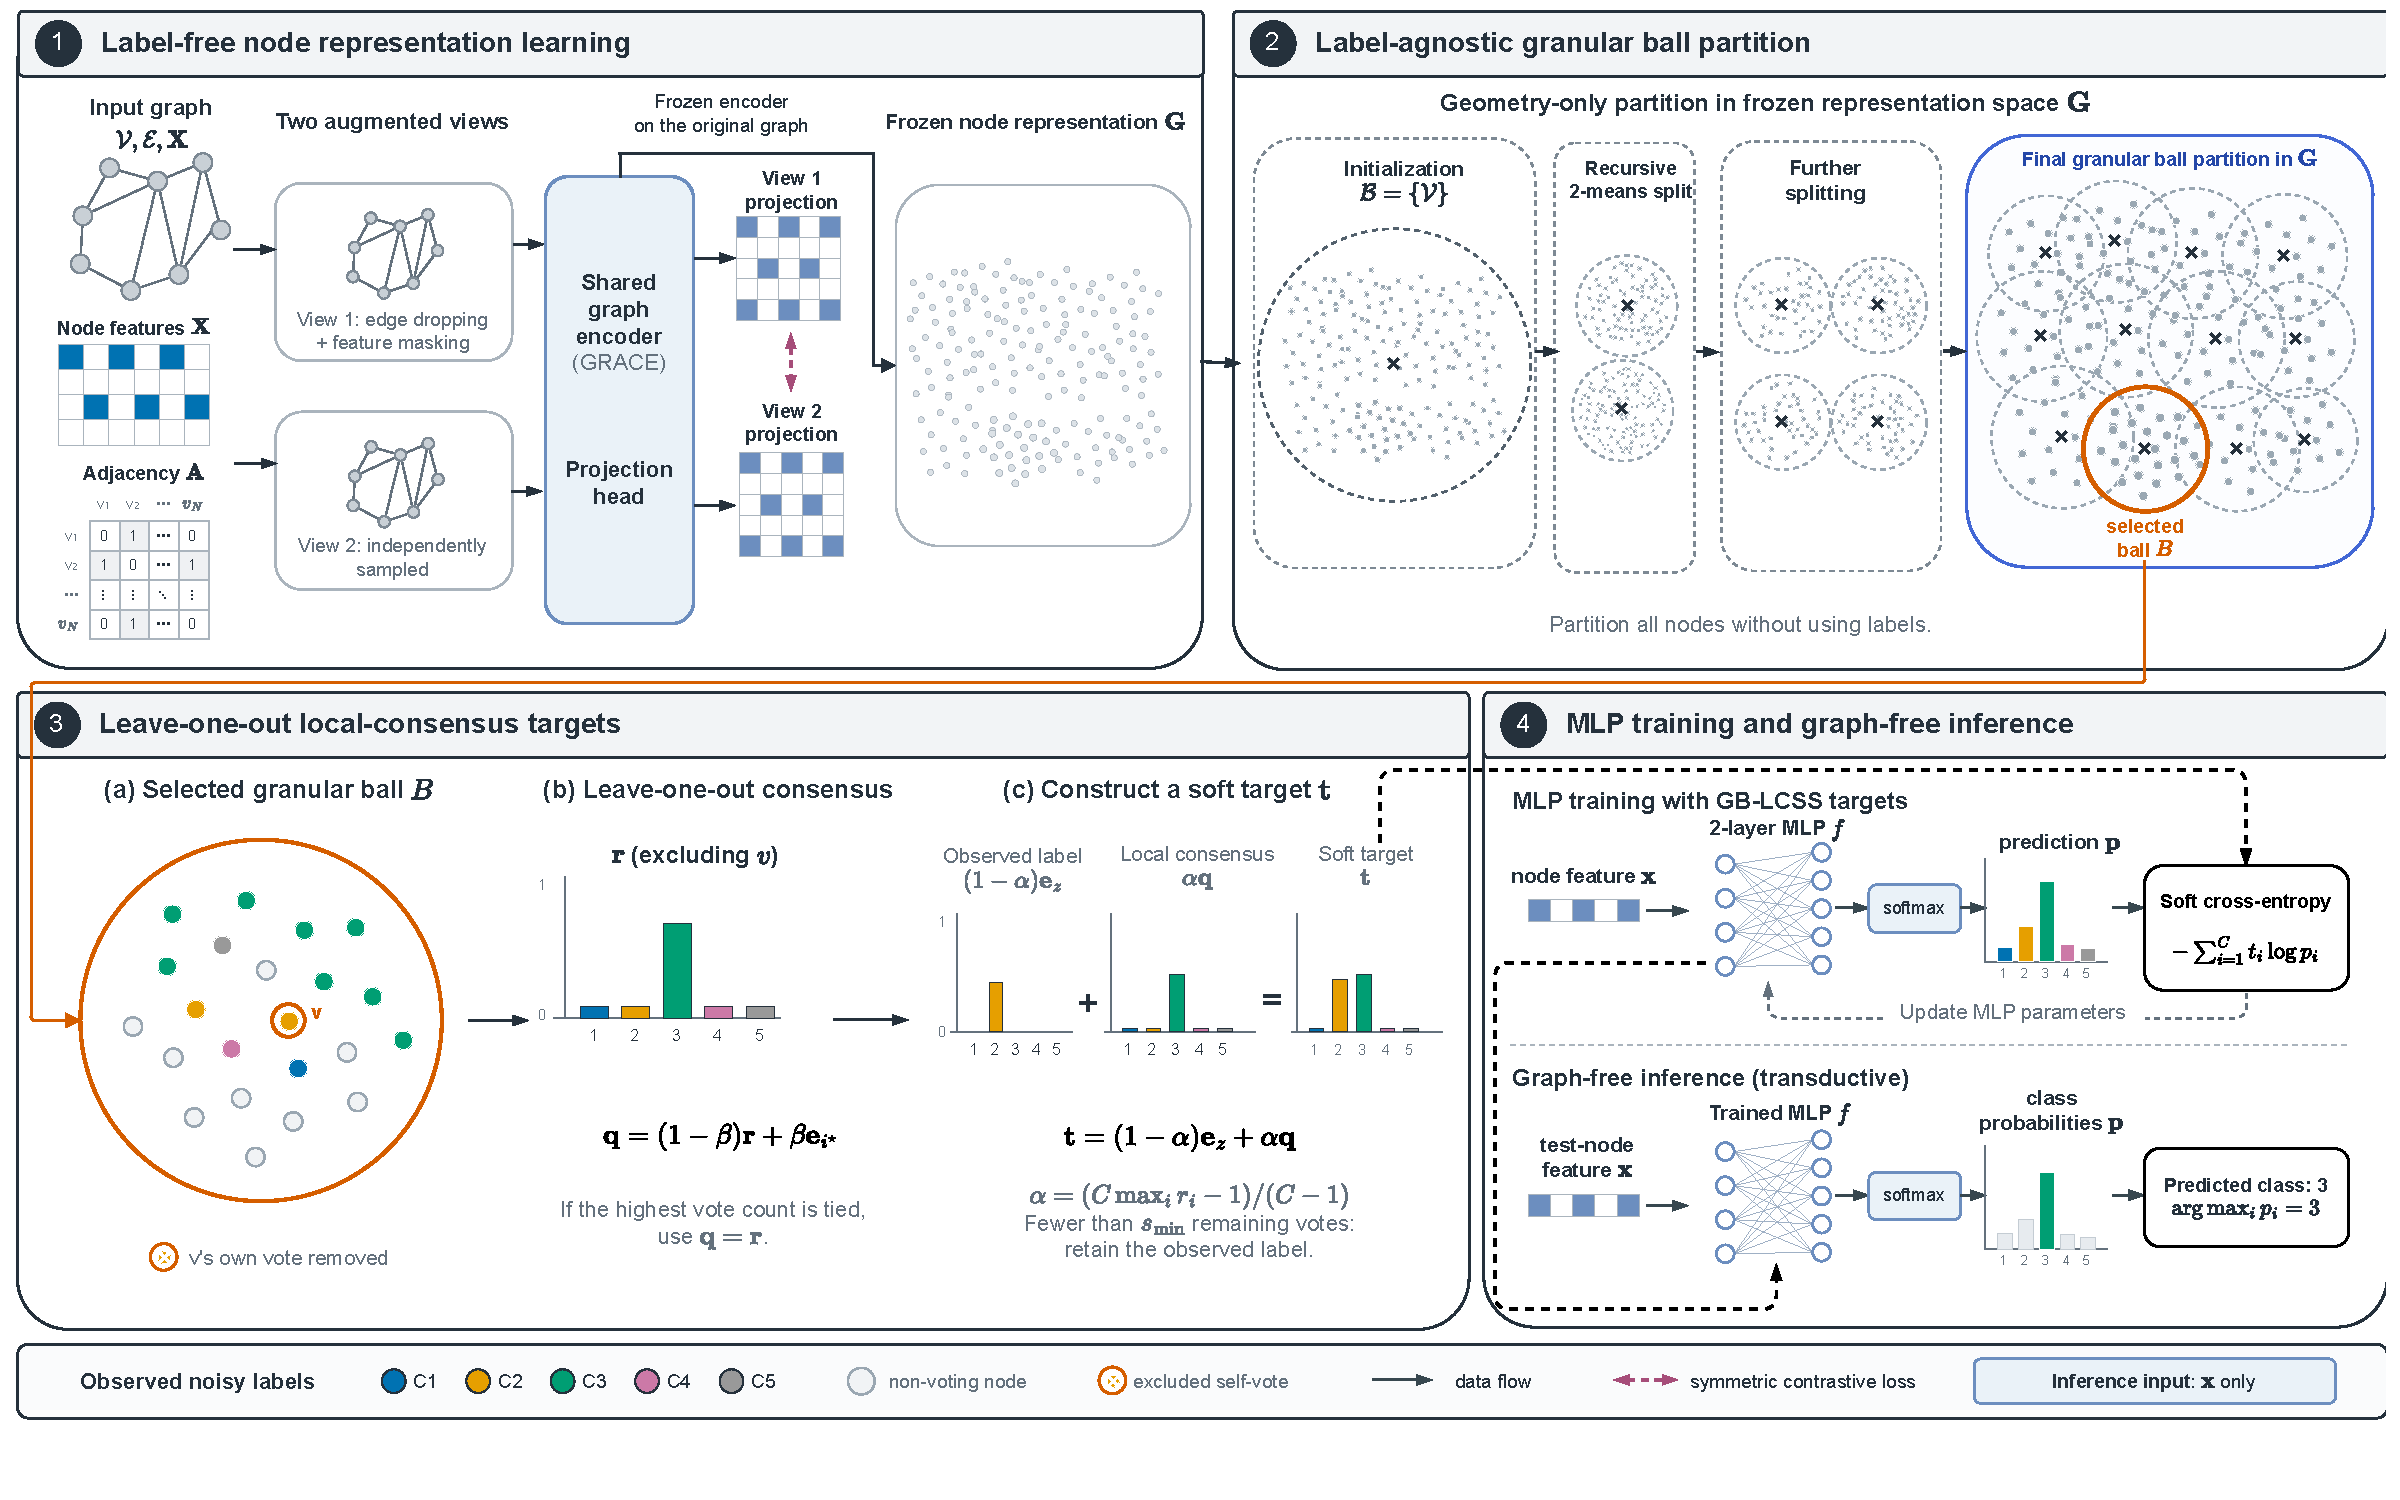
\includegraphics[width=\linewidth]{fig1.pdf}
\caption{Overview of GB-LCSS. Stage 1 learns a label-free representation, and Stage 2 constructs granular balls in that representation space. Stage 3 shows an enlarged view of a representative ball to illustrate how a local-consensus target is formed. Stage 4 trains the deployed MLP with the resulting soft targets. Hollow nodes do not vote. Ball outlines are schematic, and each node belongs to exactly one ball. For clarity, node and ball indices are omitted in the schematic.}\label{fig:1}
\end{figure}

The main contributions of this paper are summarized as follows:

\begin{enumerate}[label=(\arabic*)]
\item We introduce GB-LCSS for noisy-label node classification with graph-free inference. It organizes nodes into granular balls in a frozen, label-free graph representation, thereby separating region construction from noisy-label aggregation.
\item We construct node-specific soft targets by combining each observed label with the consensus of the other training nodes in its ball. Under independent symmetric label noise, we analyze how the number of votes and the underlying class distribution affect the reliability of local voting. We also derive an exact decomposition of the squared error of the soft target and a sufficient condition under which it has lower expected error than the observed label.
\item We evaluate GB-LCSS on five datasets under five noise settings against noisy-label learning methods and graph-assisted MLP methods. Controlled comparisons examine grouping, representation learning, target construction, and parameter sensitivity. A graph-teacher extension evaluates the same targets against graph-to-MLP distillation methods.
\end{enumerate}

The remainder of this paper is organized as follows. \hyperref[sec:2]{Section~\ref*{sec:2}} reviews related work. \hyperref[sec:3]{Section~\ref*{sec:3}} presents GB-LCSS, analyzes local-consensus supervision, and introduces the graph-teacher extension. \hyperref[sec:4]{Section~\ref*{sec:4}} describes the experimental setup, comparative results, ablation studies, extensions, and discussion. \hyperref[sec:5]{Section~\ref*{sec:5}} concludes the paper.

\section{Related work}\label{sec:2}

\subsection{Learning with noisy labels}\label{sec:2.1}

Methods for learning with noisy labels reduce the influence of corrupted annotations by selecting training samples, encouraging consistent predictions, or modifying the training objective. Sample-selection methods use the training loss to assess label reliability: Co-teaching \cite{ref17} exchanged small-loss samples between two networks, and JoCoR \cite{ref18} additionally encouraged prediction agreement. Local relationships offer another source of evidence. Deep k-NN \cite{ref11} filtered out samples whose labels disagreed with those of their neighbors, while neighbor-consistency regularization \cite{ref10} encouraged the prediction for each sample to match those of its neighbors.

Other methods address label noise by modifying the training loss. SCE \cite{ref23} combined cross-entropy with reverse cross-entropy, ELR \cite{ref24} regularized training to limit noise memorization, and LogitClip \cite{ref26} constrained logit norms. These strategies handle annotation noise without explicitly modeling graph relations between samples.

\subsection{Noise-robust learning on graphs}\label{sec:2.2}

Graph structure can provide additional evidence for assessing label reliability, while message passing may also spread the influence of supervision errors \cite{ref6}. UnionNET \cite{ref27} used neighborhood-based label estimates for reweighting and correction, NRGNN \cite{ref7} augmented supervision through structural information and pseudo-labeling, and RTGNN \cite{ref8} coordinated two networks to regulate noisy supervision.

Label reliability can also be assessed through graph topology and model behavior. TSS \cite{ref9} used topological sample selection, ProCon \cite{ref29} used peer-informed label consistency, and GNN-CFGD \cite{ref31} combined coarse- and fine-grained sample division to address label noise and sparsity.

Beyond assessing label reliability, several methods have constructed additional supervision. DND-NET \cite{ref32} used neighborhood uncertainty to reweight pseudo-label supervision, and RNCGLN \cite{ref33} combined graph contrastive learning with pseudo-graphs and pseudo-labels to address graph and label noise. Prototype-Guided Supervision \cite{ref34} formed class-level prototypes by aggregating the representations of nodes with the same observed label, while SAMTD \cite{ref36} improved supervision through multiple graph teachers.

Other methods modify neighborhood aggregation or the training objective. MILAB \cite{ref38} combined information-bottleneck-guided aggregation with adversarial consistency, and HALF \cite{ref39} fused low- and high-pass losses according to local homophily to identify reliable labels. In addition, NoisyGL \cite{ref6} established a unified evaluation framework for learning with noisy labels on graphs.

\subsection{Graph-free node classification}\label{sec:2.3}

Methods for graph-free node classification exploit graph information during training while avoiding online message passing at inference. Graph-MLP \cite{ref3} incorporated adjacency information through a neighborhood-contrastive objective, whereas GLNN \cite{ref4} distilled predictions from a GNN teacher into an MLP. Both methods deploy attribute-only MLPs. GSDN \cite{ref40} used neighborhood self-distillation, SimMLP \cite{ref41} aligned GNN and MLP representations without supervision, and SA-MLP \cite{ref44} investigated structure-aware distillation. These methods differ in how graph information guides training and in whether precomputed structural features are retained at inference.

Subsequent distillation methods differ in the teacher information they transfer. FF-G2M \cite{ref45} separated low- and high-frequency knowledge, KRD \cite{ref46} assessed knowledge reliability through the stability of prediction entropy under noise perturbations, and VQGraph \cite{ref47} encoded local structures as discrete tokens. PGKD \cite{ref48} used class prototypes to guide structural knowledge distillation from GNNs to MLPs, whereas TINED \cite{ref49} combined teacher parameter injection with Dirichlet-energy distillation. SALE-MLP \cite{ref52} investigated structure-aware latent representations. Yu et al. \cite{ref53} theoretically analyzed how label alignment in distillation allows an MLP to learn the implicit graph bias of a GNN teacher.

A related line of work uses graph structure to construct soft training targets. PosteL \cite{ref54} constructed posterior soft labels from neighborhood labels and graph-wide label statistics. ALS \cite{ref55} used neighborhood label distributions and adaptively updated smoothed targets during graph training, while SALS \cite{ref56} incorporated structural information into the target label distribution. These methods use adjacency-defined neighborhoods to construct or refine training targets. GB-LCSS also modifies the training targets, but it defines regions by proximity in a frozen, label-free representation and excludes each node's own label from the consensus that adjusts it.

\subsection{Graph contrastive representation learning}\label{sec:2.4}

Self-supervised graph learning derives training signals from node attributes and graph connectivity \cite{ref57}. Graph contrastive learning generates different views of a graph by perturbing its structure or attributes. A common node-level objective brings the representations of the same node across views closer together while distinguishing them from those of other nodes. The resulting node representations provide a basis for comparing nodes without using their observed class labels.

GRACE \cite{ref12} implements this approach through random edge dropping and feature masking, with a shared graph encoder processing the two views. Because its objective uses no class labels, GB-LCSS can compute and freeze the GRACE representation before any training label is used; the observed training labels enter only afterwards, when soft targets are constructed within the resulting groups.

\subsection{Granular ball computing}\label{sec:2.5}

Granular ball computing represents samples using coarse-grained hyperspherical regions, which GBkNN used to classify query samples \cite{ref13}. Granular ball sampling extended this representation to sample selection for noisy or imbalanced classification \cite{ref15}, and subsequent work refined adaptive ball generation \cite{ref16}. MGNR \cite{ref58} used granular ball representations to construct multi-granularity neighborhood relationships for classification and clustering.

On graphs, supervised granular ball coarsening \cite{ref66} and GBGC \cite{ref67} used granular regions to construct coarsened graphs, reducing the size of the graph on which a GNN operates. The methods above use granular regions for classification, clustering, sample selection, or graph coarsening. In supervised granular ball classifiers and sampling methods, label purity can guide ball generation \cite{ref13,ref15,ref16}. In contrast, GB-LCSS uses granular balls to organize supervision: a geometric criterion forms them in a frozen, label-free graph representation, and the observed training labels are then aggregated within each ball. Granular ball membership determines which other training nodes contribute to the soft target of each node. These targets transfer graph information into the supervision of an MLP that receives only node attributes at inference.
\section{Method}\label{sec:3}

\subsection{Problem setting and notation}\label{sec:3.1}

This subsection defines the learning task and introduces the notation used to describe GB-LCSS.

Consider an attributed graph with node set \(\mathcal V=\{v_1,\ldots,v_N\}\), edge set \(\mathcal E\subseteq\mathcal V\times\mathcal V\), adjacency matrix \(\mathbf A\in\{0,1\}^{N\times N}\), and attribute matrix \(\mathbf X=[\mathbf x_1,\ldots,\mathbf x_N]^\top\in\mathbb R^{N\times d}\), where \(\mathbf x_n\) is the attribute vector of node \(v_n\).

Each node belongs to one of \(C\geq2\) classes, indexed by \(i\in\{1,\ldots,C\}\). The set \(\mathcal V_L\subseteq\mathcal V\) contains the labeled training nodes. Node \(v_n\) has a clean label \(y_n\); if \(v_n\in\mathcal V_L\), its observed label \(z_n\) may be corrupted. Both labels take values in \(\{1,\ldots,C\}\). The method uses observed labels, whereas clean labels serve as the reference for analysis and evaluation.

To distinguish quantities associated with different objects, we use \(n\) and \(\ell\) as node indices, \(j\) as a granular ball index, and \(i\) as a class index. Bold lowercase and uppercase letters denote vectors and matrices, respectively, and calligraphic letters denote sets or collections. A second subscript selects a class component; for example, \(p_{n,i}\) is the class-\(i\) entry of the prediction vector \(\mathbf p_n\) defined below. Table~\ref{tab:notation} collects the main symbols used in the method.

\begin{table}
\centering
\caption{Main notation.}\label{tab:notation}
\small
\begin{tabular}{@{}p{0.27\linewidth}p{0.70\linewidth}@{}}
\toprule
Symbol & Meaning \\
\midrule
\multicolumn{2}{@{}l}{\textit{Graph and data}} \\
\(\mathcal V,\mathcal E\) & Node set and edge set \\
\(N,C\) & Number of nodes and number of classes \\
\(n,\ell\) & Node indices in \(\{1,\ldots,N\}\) \\
\(j\) & Granular ball index \\
\(i\) & Class index in \(\{1,\ldots,C\}\) \\
\(\mathbf A,\mathbf X\) & Adjacency matrix and node attribute matrix \\
\(\mathbf x_n\) & Attribute vector of node \(v_n\) \\
\(\mathcal V_L\) & Set of labeled training nodes \\
\(y_n,z_n\) & Clean and observed labels of node \(v_n\) \\
\(\eta\) & Label corruption probability \\
\midrule
\multicolumn{2}{@{}l}{\textit{Representations and granular balls}} \\
\(\mathbf G,\mathbf g_n\) & Frozen normalized GRACE representation matrix and vector for node \(v_n\) \\
\(d,h\) & Attribute dimension and GRACE representation dimension \\
\(\mathcal B,B_j\) & Collection of granular balls and its \(j\)-th member \\
\(\boldsymbol\mu_j,D(B_j)\) & Center and mean radius of ball \(B_j\) \\
\(D'(B_j)\) & Size-weighted mean radius after splitting \(B_j\) \\
\(B_{\max}\) & Maximum number of granular balls \\
\(n_{\min}\) & Minimum number of nodes in each accepted child ball \\
\(\delta\) & Minimum relative decrease in mean radius for an accepted split \\
\midrule
\multicolumn{2}{@{}l}{\textit{Local consensus and soft targets}} \\
\(\mathbf w_j\) & Observed class-count vector of training nodes in \(B_j\) \\
\(U_n\) & Other training nodes in the ball containing \(v_n\) \\
\(s_{\min}\) & Minimum number of votes required to use local consensus \\
\(\mathbf r_n\) & Observed class proportions among the voting nodes in \(U_n\) \\
\(i_n^\star\) & Class with the unique highest vote count in \(U_n\) \\
\(\mathbf q_n\) & Local-consensus class distribution for node \(v_n\) \\
\(\beta\) & Strength of the adjustment toward the uniquely most-voted class \\
\(\alpha_n\) & Weight of the local consensus in the target for \(v_n\) \\
\(\mathbf e_i,\mathbb I(\cdot)\) & One-hot vector for class \(i\); indicator function \\
\(\mathbf t_n\) & Soft training target for node \(v_n\) \\
\(f,\mathbf p_n\) & MLP classifier and its predicted class distribution for \(v_n\) \\
\bottomrule
\end{tabular}
\end{table}


During training, the complete \(\mathbf X\) and \(\mathbf A\), including the attributes and topology of test nodes, are available for label-free representation learning and target construction, while test labels remain hidden. The goal is to learn an MLP \(f\) whose predicted class distribution for node \(v_n\) is
\begin{equation}\label{eq:1}
\mathbf p_n=\operatorname{softmax}\bigl(f(\mathbf x_n)\bigr).
\end{equation}
Here, \(p_{n,i}\) is the predicted probability that node \(v_n\) belongs to class \(i\). After training, only \(f\) is retained for inference.

\subsection{Label-free representation learning and granular ball construction}\label{sec:3.2}

GB-LCSS first learns a label-free graph representation and then uses its geometry to partition the nodes into granular balls.

\subsubsection{Label-free representation learning}\label{sec:3.2.1}

\enlargethispage{\baselineskip}
We pretrain GRACE \cite{ref12} on the node attributes and graph connectivity without class labels and then freeze the encoder. For distance-based grouping, we take the encoder output before the projection head and normalize each node representation. The resulting GRACE representation matrix is
\begin{equation}\label{eq:2}
\mathbf G=[\mathbf g_1,\ldots,\mathbf g_N]^\top\in\mathbb R^{N\times h},
\end{equation}
where \(\mathbf g_n\) is the normalized representation of the \(n\)-th node and \(h\) is the representation dimension. Let \(\mathbf g'_n\) denote the encoder output for node \(v_n\) before normalization. Its normalized representation is
\begin{equation}\label{eq:3}
\mathbf g_n=\frac{\mathbf g'_n}{\max(\|\mathbf g'_n\|_2,\varepsilon)}.
\end{equation}
Here, \(\|\cdot\|_2\) denotes the Euclidean norm, and \(\varepsilon=10^{-12}\) is a numerical safeguard. The same row-wise normalization is applied to all nodes to form \(\mathbf G\). \hyperref[sec:4.3.3]{Section~\ref*{sec:4.3.3}} examines alternative representations and the variation across GRACE pretraining seeds.

\subsubsection{Granular ball construction}\label{sec:3.2.2}

We denote the collection of granular balls constructed from \(\mathbf G\) by \(\mathcal B=\{B_1,\ldots,B_M\}\), where \(B_j\) is the \(j\)-th ball, a subset of \(\mathcal V\), and \(M\) is the final number of balls. Each node is assigned to exactly one ball, whose training nodes provide local label evidence. Construction starts with \(\mathcal B=\{\mathcal V\}\) and recursively splits its member balls. To decide whether a split improves the grouping, we first measure how tightly the node representations in a ball are concentrated around its center.

\begin{definition}
For a nonempty granular ball \(B_j\), each member node \(v_n\in B_j\) has the normalized representation \(\mathbf g_n\). The center \(\boldsymbol\mu_j\) and mean radius \(D(B_j)\) of the ball are
\begin{equation}\label{eq:4}
\boldsymbol\mu_j=\frac{1}{|B_j|}\sum_{v_n\in B_j}\mathbf g_n,
\qquad D(B_j)=\frac{1}{|B_j|}\sum_{v_n\in B_j}\|\mathbf g_n-\boldsymbol\mu_j\|_2.
\end{equation}
\end{definition}

The mean radius is the average Euclidean distance from the member representations to the ball center. A smaller value indicates a more compact ball.


Let \(n_{\min}\) be a positive integer denoting the minimum number of nodes allowed in each child ball. A ball \(B_j\) in the current collection is eligible for splitting only if \(|B_j|\geq 2n_{\min}\). Eligible balls are examined in descending order of \(D(B_j)\), so that more dispersed balls are considered first. For each candidate ball \(B_j\), 2-means produces two child balls \(B_j^{(1)}\) and \(B_j^{(2)}\).

\begin{definition}
The size-weighted post-split dispersion of \(B_j\) is
\begin{equation}\label{eq:5}
D'(B_j) = \frac{|B_j^{(1)}|D(B_j^{(1)}) + |B_j^{(2)}|D(B_j^{(2)})}{|B_j|}.
\end{equation}
Let \(\delta \in (0,1)\) specify the minimum relative decrease in the mean radius. The split is accepted only if both child balls contain at least \(n_{\min}\) nodes and
\begin{equation}\label{eq:6}
D'(B_j) \leq (1 - \delta)D(B_j).
\end{equation}
\end{definition}

Weighting the child radii by their sizes makes \(D'(B_j)\) the average distance from the same nodes to their new centers, so Eq.~\eqref{eq:6} requires this average to decrease by at least a fraction \(\delta\). We accept the first candidate split that satisfies both conditions, update the ball collection, and reorder the remaining candidates.

Splitting stops when no valid candidate remains or when the number of balls reaches the maximum permitted number \(B_{\max}\), so that \(M\leq B_{\max}\). \hyperref[sec:4.1.4]{Section~\ref*{sec:4.1.4}} gives the experimental values of the partition parameters, and Algorithm~\ref{alg:1} summarizes the procedure. Its Boolean flag \(\mathrm{accepted}\) records whether a split has been accepted in the current pass; if no split is accepted, construction stops.

\begin{algorithm}
\caption{Recursive granular ball partitioning in the frozen representation space}\label{alg:1}
\KwIn{Normalized frozen representation $\mathbf G$, node set $\mathcal V$, parameters $B_{\max},n_{\min},\delta$}
\KwOut{Granular ball partition $\mathcal B$}
$\mathcal B\gets\{\mathcal V\}$\;
\While{$|\mathcal B|<B_{\max}$}{
  $\mathrm{accepted}\gets\mathrm{false}$\;
  \ForEach{$B_j\in\mathcal B$ with $|B_j|\ge 2n_{\min}$, in descending order of $D(B_j)$}{
    Apply 2-means to the normalized representations of nodes in $B_j$ to obtain $B_j^{(1)}$ and $B_j^{(2)}$\;
    \If{$\min(|B_j^{(1)}|,|B_j^{(2)}|)\ge n_{\min}$ and $D'(B_j)\le(1-\delta)D(B_j)$}{
      $\mathcal B\gets(\mathcal B\setminus\{B_j\})\cup\{B_j^{(1)},B_j^{(2)}\}$\;
      $\mathrm{accepted}\gets\mathrm{true}$\;
      \KwBreak\;
    }
  }
  \If{$\mathrm{accepted}=\mathrm{false}$}{\KwBreak\;}
}
\KwRet $\mathcal B$\;
\end{algorithm}


\subsection{Local-consensus supervision and MLP training}\label{sec:3.3}

Given the partition, GB-LCSS constructs each training target by summarizing the observed labels of the other training nodes in the same ball and combining their consensus with the node's own observed label. These targets then supervise MLP training.

\subsubsection{Within-ball label consensus}\label{sec:3.3.1}

Consider a training node \(v_n\) and the granular ball \(B_j\) containing it. We construct its target using a leave-one-out vote that excludes \(v_n\), and repeat this calculation for every training node.

\begin{definition}
The voting set \(U_n\) contains the other training nodes in \(B_j\):
\begin{equation}\label{eq:7}
U_n=(B_j\cap\mathcal V_L)\setminus\{v_n\}.
\end{equation}
Let \(s_{\min}\geq1\) be an integer specifying the minimum number of voting nodes required to use local consensus. When \(|U_n|\geq s_{\min}\), the observed labels of the voting nodes define the empirical class distribution \(\mathbf r_n=(r_{n,1},\ldots,r_{n,C})^\top\), with
\begin{equation}\label{eq:8}
r_{n,i}=\frac{1}{|U_n|}\sum_{v_\ell\in U_n}\mathbb I(z_\ell=i),
\qquad i=1,\ldots,C.
\end{equation}
\end{definition}

Here, \(z_\ell\) is the observed label of voting node \(v_\ell\), and \(\mathbb I(z_\ell=i)\) equals one if this label is \(i\) and zero otherwise. The entries of \(\mathbf r_n\) are nonnegative and sum to one. Excluding \(v_n\) prevents its observed label from reinforcing the consensus used to adjust it.

\begin{definition}
If a single class receives more votes than every other class, its index is
\begin{equation}\label{eq:9}
i_n^\star=\operatorname*{arg\,max}_i r_{n,i}.
\end{equation}
The local-consensus distribution \(\mathbf q_n\) assigns additional weight to this class through the parameter \(\beta\in[0,1]\):
\begin{equation}\label{eq:10}
\mathbf q_n=
\begin{cases}
(1-\beta)\mathbf r_n+\beta\mathbf e_{i_n^\star},&\text{if a unique highest-vote class exists}\\
\mathbf r_n,&\text{if the highest vote count is tied},
\end{cases}
\end{equation}
\end{definition}

Here, \(\mathbf e_i\) is the one-hot vector with value 1 at class \(i\) and 0 elsewhere. The parameter \(\beta\) controls the weight assigned to the one-hot distribution of the uniquely most-voted class.

\subsubsection{Consensus-weighted soft targets}\label{sec:3.3.2}

The distribution \(\mathbf q_n\) summarizes the observed labels of the other training nodes. Its weight in the final target is determined by the largest class proportion in the original vote distribution \(\mathbf r_n\).

\begin{definition}
When \(|U_n|\geq s_{\min}\), the consensus weight \(\alpha_n\) is defined by rescaling the largest vote proportion relative to the uniform class probability \(1/C\):
\begin{equation}\label{eq:11}
\alpha_n=\frac{C\max_i r_{n,i}-1}{C-1}.
\end{equation}
\end{definition}

Because \(\mathbf r_n\) is a class distribution, its largest entry lies between \(1/C\) and 1. Equation~\eqref{eq:11} maps this interval onto \([0,1]\): uniformly distributed votes give \(\alpha_n=0\), and unanimous votes give \(\alpha_n=1\). For fixed votes, changing \(\beta\) leaves \(\alpha_n\) unchanged.

\begin{definition}
The soft target \(\mathbf t_n\) combines the observed label of \(v_n\) with its local consensus:
\begin{equation}\label{eq:12}
\mathbf t_n=
\begin{cases}
(1-\alpha_n)\mathbf e_{z_n}+\alpha_n\mathbf q_n,&|U_n|\geq s_{\min}\\
\mathbf e_{z_n},&|U_n|<s_{\min},
\end{cases}
\end{equation}
\end{definition}

The target is a convex combination of the observed one-hot label and local consensus, with \(\alpha_n\) controlling the consensus contribution. Nodes with fewer than \(s_{\min}\) other training nodes in their ball retain their observed one-hot labels.

Equations~\eqref{eq:7}--\eqref{eq:12} use only the observed labels of training nodes; validation and test labels are not used in target construction. For each ball \(B_j\), Algorithm~\ref{alg:2} stores the observed class counts of its training nodes in a vector \(\mathbf w_j\). For each training node \(v_n\in B_j\), it subtracts the node's own vote from \(\mathbf w_j\) and constructs \(\mathbf t_n\) from the remaining counts.

\begin{algorithm}
\caption{Granular ball soft-target construction}\label{alg:2}
\KwIn{Granular ball partition $\mathcal B$, training nodes $\mathcal V_L$, observed labels $\{z_n:v_n\in\mathcal V_L\}$, number of classes $C$, parameters $s_{\min},\beta$}
\KwOut{One stored soft target for each node in $\mathcal V_L$}
Initialize $\mathbf t_n\gets\mathbf e_{z_n}$ for every training node $v_n\in\mathcal V_L$\;
\ForEach{$B_j\in\mathcal B$}{
  $\mathbf w_j\gets\sum_{v_\ell\in B_j\cap\mathcal V_L}\mathbf e_{z_\ell}$\;
  \ForEach{$v_n\in B_j\cap\mathcal V_L$}{
    $U_n\gets(B_j\cap\mathcal V_L)\setminus\{v_n\}$\;
    \If{$|U_n|<s_{\min}$}{continue\;}
    $\mathbf r_n\gets(\mathbf w_j-\mathbf e_{z_n})/|U_n|$\;
    \eIf{one class $i_n^\star$ has a strictly larger vote count than every other class}{
      $\mathbf q_n\gets(1-\beta)\mathbf r_n+\beta\mathbf e_{i_n^\star}$\;
    }{
      $\mathbf q_n\gets\mathbf r_n$\;
    }
    $\alpha_n\gets(C\max_i r_{n,i}-1)/(C-1)$\;
    $\mathbf t_n\gets(1-\alpha_n)\mathbf e_{z_n}+\alpha_n\mathbf q_n$\;
  }
}
\KwRet Stored targets for all nodes in $\mathcal V_L$\;
\end{algorithm}


\subsubsection{MLP training}\label{sec:3.3.3}

The two-layer MLP \(f\) consists of a hidden linear layer, followed by ReLU, batch normalization, and dropout, and an output layer that produces class logits. The training loss is
\begin{equation}\label{eq:13}
\mathcal L=-\frac{1}{|\mathcal V_L|}\sum_{v_n\in\mathcal V_L}\sum_{i=1}^C t_{n,i}\log p_{n,i}.
\end{equation}

\subsection{Analysis of local-consensus supervision}\label{sec:3.4}

Under independent symmetric label noise, we bound the local-vote error probability and derive a sufficient condition for a lower expected soft-target error. The partition, the training-node set, and the clean labels are fixed. Let \(\eta\) denote the corruption probability: each label is independently retained with probability \(1-\eta\) and otherwise replaced by a uniformly chosen incorrect class.

Fix a training node \(v_n\) with clean label \(y_n\) and \(s_n=|U_n|\geq s_{\min}\) voting nodes. The clean class proportions and the margin of the true class over its closest competitor are
\begin{equation}\label{eq:14}
a_{n,i}=\frac{1}{s_n}\sum_{v_\ell\in U_n}\mathbb I(y_\ell=i),
\qquad
\Delta_n=a_{n,y_n}-\max_{i\ne y_n}a_{n,i}.
\end{equation}
Here, \(a_{n,i}\) is the fraction of nodes in \(U_n\) whose clean label is \(i\), and \(a_{n,y_n}\) selects the proportion for the true class of \(v_n\). A positive \(\Delta_n\) means that this class receives more clean votes than any competing class. We use \(\Pr\) to denote probability over the independent label corruptions.

\begin{proposition}\label{prop:local_vote}
Suppose that \(C\geq2\), \(\Delta_n>0\), and \(0\leq\eta<(C-1)/C\), and let \(\gamma=1-C\eta/(C-1)>0\). Each voting label is independently flipped with probability \(\eta\) to a uniformly chosen incorrect class. Then
\begin{equation}\label{eq:15}
\Pr\!\left(\max_{i\ne y_n}r_{n,i}\geq r_{n,y_n}\right)
\leq\min\!\left\{1,(C-1)\exp\!\left(-\frac{s_n\gamma^2\Delta_n^2}{2}\right)\right\}.
\end{equation}
\end{proposition}

\begin{proof}
\renewcommand{\qedsymbol}{}
Fix a competing class \(i\ne y_n\). For each voting node \(v_\ell\in U_n\), define \(\xi_\ell=\mathbb I(z_\ell=y_n)-\mathbb I(z_\ell=i)\). These variables are independent and lie in \([-1,1]\), and their average is \(\bar\xi=r_{n,y_n}-r_{n,i}\). Under symmetric label corruption,
\[
\mathbb E[\bar\xi]=\gamma(a_{n,y_n}-a_{n,i})\geq\gamma\Delta_n.
\]
Hoeffding's inequality \cite{hoeffding1963} therefore gives
\[
\Pr\!\left(r_{n,i}\geq r_{n,y_n}\right)=\Pr(\bar\xi\leq0)
\leq\exp\!\left(-\frac{s_n\gamma^2\Delta_n^2}{2}\right).
\]
Taking the union bound over the \(C-1\) competing classes and capping the bound at one yields Eq.~\eqref{eq:15}.
\end{proof}

Symmetric corruption reduces the expected margin over the closest competitor from \(\Delta_n\) to \(\gamma\Delta_n\). For a fixed positive margin and noise rate, the exponential term in the bound decreases as the number of votes increases. However, enlarging a group can also change its class composition and reduce the margin, so both quantities matter for voting reliability. The adjustment in Eq.~\eqref{eq:10} preserves the most-voted classes, and the same bound therefore applies to \(\mathbf q_n\). Appendix~H.1 in the Supplementary Material gives the detailed expectation calculation.

Proposition~1 bounds the probability that local voting fails to give the true class a unique lead. We next assess the full soft-target distribution through its squared distance from the clean one-hot label. For node \(v_n\), \(\mathbf e_{z_n}\) is its observed one-hot label. The Brier score of a target vector \(\mathbf b\) is \(\operatorname{BS}_n(\mathbf b)=\|\mathbf b-\mathbf e_{y_n}\|_2^2\). The target \(\mathbf t_n=(1-\alpha_n)\mathbf e_{z_n}+\alpha_n\mathbf q_n\) satisfies
\begin{equation}\label{eq:16}
\operatorname{BS}_n(\mathbf t_n)=(1-\alpha_n)\operatorname{BS}_n(\mathbf e_{z_n})+\alpha_n\operatorname{BS}_n(\mathbf q_n)-\alpha_n(1-\alpha_n)\|\mathbf e_{z_n}-\mathbf q_n\|_2^2.
\end{equation}
This identity expresses the error of the soft target as the weighted sum of the errors of the observed label and the local consensus, minus a nonnegative term determined by their disagreement. The following corollary gives a sufficient condition for an improvement in expectation.

\begin{corollary}\label{cor:expected}
For the fixed node \(v_n\) with \(|U_n|\geq s_{\min}\), assume independent symmetric label corruption with rate \(\eta\). Fix the partition, the training-node set, the clean labels, and the observed labels of all other training nodes. Then \(\mathbf q_n\) and \(\alpha_n\) are fixed, and
\begin{equation}\label{eq:17}
\mathbb E[\operatorname{BS}_n(\mathbf t_n)]\leq2\eta(1-\alpha_n)+\alpha_n\operatorname{BS}_n(\mathbf q_n),
\end{equation}
where the expectation is taken over the corruption of node \(v_n\)'s label. If \(\alpha_n>0\) and \(\operatorname{BS}_n(\mathbf q_n)<2\eta\), the soft target has a lower expected squared error than the observed one-hot label.
\end{corollary}

Because node \(v_n\) is excluded from its own vote, \(\mathbf q_n\) and \(\alpha_n\) do not change with its observed label, whose one-hot vector has expected squared error \(2\eta\). Taking the expectation of Eq.~\eqref{eq:16} and omitting its nonpositive final term therefore gives Eq.~\eqref{eq:17} (Appendix~H.2). The condition compares the error of the consensus distribution with the expected error of a noisy annotation.

Across the training set, the change in Brier score combines the error reduction on corrupted labels with any error introduced on correct labels. Section~\ref{sec:4.3.1} reports the net reduction, and Appendix~I.2 measures the two components separately.

\subsection{Graph-teacher distillation extension}\label{sec:3.5}

The base method trains the MLP on the labeled training nodes. In the extension, the same targets supervise a GCN teacher, whose predictions on all nodes are distilled into an MLP student.

The teacher is a two-layer GCN that takes the original attributes \(\mathbf X\) and the adjacency matrix \(\mathbf A\) as inputs. Its class-logit matrix is
\begin{equation}\label{eq:18}
\mathbf O=\operatorname{GCN}(\mathbf X,\mathbf A)\in\mathbb R^{N\times C}.
\end{equation}
Let \(\mathbf o_n\in\mathbb R^C\) denote the teacher-logit vector for node \(v_n\), whose transpose is the \(n\)-th row of \(\mathbf O\). The teacher loss is
\begin{equation}\label{eq:19}
\mathcal L_1=-\frac{1}{|\mathcal V_L|}\sum_{v_n\in\mathcal V_L}\sum_{i=1}^C t_{n,i}\log\bigl[\operatorname{softmax}(\mathbf o_n)\bigr]_i.
\end{equation}
The teacher therefore uses \(\mathbf G\) only through the GB-LCSS targets; its inputs are \(\mathbf X\) and \(\mathbf A\).

After checkpoint selection, the teacher is frozen. With distillation temperature \(\tau>0\), its prediction for node \(v_n\) is
\begin{equation}\label{eq:20}
\boldsymbol\pi_n=\operatorname{softmax}\left(\frac{\mathbf o_n}{\tau}\right).
\end{equation}
Here, \(\pi_{n,i}\) is the teacher's probability for class \(i\) at node \(v_n\). Increasing \(\tau\) produces a softer distribution. The resulting distribution is stored as the distillation target of the node.

The MLP student \(f\) is trained on all \(N\) nodes, with these distributions as its sole distillation targets. Its loss is
\begin{equation}\label{eq:21}
\mathcal L_2=-\frac{\tau^2}{N}\sum_{n=1}^{N}\sum_{i=1}^C\pi_{n,i}
\log\left[\operatorname{softmax}\left(\frac{f(\mathbf x_n)}{\tau}\right)\right]_i.
\end{equation}
After distillation, only the MLP student is retained for inference on node attributes.

\subsection{Computational costs}\label{sec:3.6}

Relative to direct MLP training, GB-LCSS adds three training-time stages: graph contrastive pretraining, granular ball partitioning, and soft-target construction. The pretraining cost depends on the encoder and the training schedule; \hyperref[sec:4.4.2]{Section~\ref*{sec:4.4.2}} reports the measured cost. Pretraining is shared across downstream runs that use the same frozen representation.


The cost of partitioning is dominated by the 2-means calls. Running 2-means for \(I\) iterations on a ball \(B_j\), with a fixed number of initializations, costs \(\mathcal{O}(I\,|B_j|\,h)\). The candidate balls examined in one pass of Algorithm~\ref{alg:1} are disjoint, so their combined size is at most \(N\). Each pass either accepts one split or terminates the algorithm. There are at most \(B_{\max}-1\) successful passes and one final unsuccessful pass, so the total cost of all 2-means calls is bounded by

\begin{equation}\label{eq:22}
\mathcal{O}(I\,B_{\max}\,N\,h).
\end{equation}

For fixed \(I\) and \(B_{\max}\), this bound is linear in both the number of nodes and the representation dimension. Sorting the candidates by dispersion in each pass adds at most \(\mathcal{O}(B_{\max}^{2}\log B_{\max})\) operations in total. The frozen representation \(\mathbf G\) requires \(\mathcal{O}(Nh)\) space, and the node assignments, ball centers, and per-ball class counts require \(\mathcal{O}(N + B_{\max}(h + C))\) space. Given the per-ball class counts, computing the targets for the labeled nodes takes \(\mathcal{O}(|\mathcal{V}_{L}|C)\) time. The implementation initializes and stores a dense \(N \times C\) target matrix, which adds \(\mathcal{O}(NC)\) time and space.


The classifier is the same two-layer MLP as that used in the baselines. Let \(F\) denote its hidden width and \(T_{S}\) the number of training epochs. The loss in Eq.~\eqref{eq:13} involves only the training nodes, but the full-batch implementation evaluates all \(N\) nodes in each epoch, at a total cost of \(\mathcal{O}(T_{S}N(dF + FC))\). At inference, the cost per node is

\begin{equation}\label{eq:23}
\mathcal{O}(dF + FC).
\end{equation}

The model parameters also require \(\mathcal{O}(dF + FC)\) space. The extension additionally trains a GCN teacher and then trains an MLP student on the teacher's predictions for all \(N\) nodes. Its deployed MLP has the same architecture and inference cost as above.
\section{Experiments}\label{sec:4}

\subsection{Experimental setup}\label{sec:4.1}

\subsubsection{Datasets}\label{sec:4.1.1}

The main experiments use five public datasets: the citation graphs Cora and CiteSeer \cite{ref69}, the 70-class citation graph CoraFull, the co-authorship graph Coauthor-CS, and the co-purchase graph Amazon-Photo \cite{ref70}. Table~\ref{tab:1} summarizes their statistics. Edges are counted as unique undirected pairs after self-loop removal, training-node counts refer to the 20\% split, and edge homophily is the proportion of edges that connect nodes of the same class. Six additional datasets are evaluated under uniform 0.4 noise (Appendix~G).

\begin{table}
\centering
\caption{Statistics of the five main datasets.}\label{tab:1}
\begingroup
\fontsize{9}{11}\selectfont
\setlength{\tabcolsep}{3pt}
\renewcommand{\arraystretch}{1.18}
\setlength{\TableWidth}{\dimexpr\linewidth-12\tabcolsep\relax}
\begin{tabular}{@{}>{\raggedright\arraybackslash}p{\dimexpr 0.200000\TableWidth\relax}>{\centering\arraybackslash}p{\dimexpr 0.111111\TableWidth\relax}>{\centering\arraybackslash}p{\dimexpr 0.166667\TableWidth\relax}>{\centering\arraybackslash}p{\dimexpr 0.111111\TableWidth\relax}>{\centering\arraybackslash}p{\dimexpr 0.100000\TableWidth\relax}>{\centering\arraybackslash}p{\dimexpr 0.155556\TableWidth\relax}>{\centering\arraybackslash}p{\dimexpr 0.155556\TableWidth\relax}@{}}
\toprule
\textbf{Dataset} & \textbf{Nodes} & \textbf{Undirected edges} & \textbf{Features} & \textbf{Classes} & \textbf{Training nodes} & \textbf{Edge homophily} \\
\midrule
Cora & 2,708 & 5,278 & 1,433 & 7 & 541 & 0.810 \\
CiteSeer & 3,327 & 4,552 & 3,703 & 6 & 665 & 0.736 \\
CoraFull & 19,793 & 63,421 & 8,710 & 70 & 3,958 & 0.567 \\
Coauthor-CS & 18,333 & 81,894 & 6,805 & 15 & 3,666 & 0.808 \\
Amazon-Photo & 7,650 & 119,081 & 745 & 8 & 1,530 & 0.827 \\
\bottomrule
\end{tabular}
\endgroup
\end{table}


\subsubsection{Data splits and label noise}\label{sec:4.1.2}

All comparisons follow the fixed-graph transductive protocol of \hyperref[sec:3.1]{Section~\ref*{sec:3.1}}. For each seed from 0 to 4, we use the NoisyGL percentage-split routine to randomly sample training, validation, and test nodes from the full node set at ratios of 20\%, 10\%, and 70\%, respectively. Noise is injected only into the training labels, and all methods share the same split and noisy labels for each dataset and seed. Clean validation labels are used for checkpoint selection, and test labels for final evaluation. Appendix~F gives the exact subset sizes and the sampling procedure, and Appendix~C examines sensitivity to corrupted validation labels.

Under uniform noise, each training label is retained with probability \(1-\eta\) and is replaced by each of the other \(C-1\) classes with probability \(\eta/(C-1)\). We evaluate \(\eta\in\{0.2,0.4,0.6\}\). Pair noise uses \(\eta=0.4\): it changes class \(i\in\{1,\ldots,C\}\) to \(((i-2)\bmod C)+1\) with probability \(\eta\) and leaves it unchanged with probability \(1-\eta\). Instance-dependent noise is generated with the NoisyGL generator, using a configured mean flip rate of 0.4 and \(\text{norm\_std}=0.1\).

\subsubsection{Compared methods}\label{sec:4.1.3}

The first comparison group comprises seven noisy-label baselines: MLP+CE, Small-loss, Co-teaching, JoCoR, SCE, ELR, and LogitClip. They use the same deployed two-layer MLP and the same labeled training nodes as GB-LCSS. GB-LCSS uses graph information during training and requires no noise-model parameters. Small-loss, Co-teaching, and JoCoR use the true noise rate to set their forget-rate schedules. Small-loss selects samples by their per-sample cross-entropy. Co-teaching and JoCoR train two independently initialized MLPs but evaluate a single network without ensembling.

The second group comprises graph-assisted MLP methods: PosteL \cite{ref54}, ALS \cite{ref55}, SALS \cite{ref56}, Graph-MLP \cite{ref3}, and GSDN \cite{ref40}. All of them use graph information only during training in our protocol. PosteL uses the official target-construction code with iterative pseudo-labeling disabled. Graph-MLP is adapted to the common MLP, whereas ALS, SALS, and GSDN are implemented as mechanism adaptations under the common protocol. Appendix~F identifies the retained components and parameter sources for each method.

The third group comprises graph-to-MLP distillation methods: a GCN(X)+CE response-distillation baseline based on GLNN \cite{ref4}, FF-G2M \cite{ref45}, KRD \cite{ref46}, VQGraph \cite{ref47}, and a GCN teacher trained on GB-LCSS targets (\hyperref[sec:3.5]{Section~\ref*{sec:3.5}}). FF-G2M is reimplemented with the common backbones and its low- and high-frequency objectives. The mechanism adaptations of KRD and VQGraph retain reliability-based knowledge selection and soft-codebook distillation, respectively. For each seed, the teacher and student are retrained for every route, using the same MLP configuration for all students.

\subsubsection{Implementation details}\label{sec:4.1.4}

Datasets are loaded through the NoisyGL interface to PyTorch Geometric. Graph contrastive pretraining uses row-normalized attributes, whereas downstream models use the attributes supplied by NoisyGL. Graph-convolutional models use the supplied adjacency, with normalization and self-loops handled within their graph-convolution layers.

The noisy-label baselines and GB-LCSS use a two-layer MLP with a hidden width of 64 and a dropout rate of 0.5. We train for 200 epochs using Adam with a learning rate of 0.01 and a weight decay of \(5 \times 10^{- 4}\), and we select the checkpoint with the highest validation accuracy. Teacher checkpoints are selected with the same criterion.

By default, GB-LCSS uses \(B_{\max} = 64\), \(n_{\min} = 32\), \(\delta = 0.05\), \(s_{\min} = 2\), and \(\beta = 0.5\). Recursive 2-means uses Euclidean distance, k-means++ initialization \cite{ref71}, and 10 initializations per candidate split, with randomization controlled by the downstream seed. The distillation extension uses a temperature of \(\tau = 1\). GRACE configurations and all other parameter settings, with their sources, are given in Appendix~F.

\subsubsection{Evaluation protocol}\label{sec:4.1.5}

Test-node classification accuracy is reported in percent as the mean \ensuremath{\pm} sample standard deviation over five paired seeds. Bold marks the highest mean within each dataset and noise setting; in Table~\ref{tab:3}, underlining marks the second-highest mean. Each dataset uses one fixed normalized pretrained representation \(\mathbf G\). \hyperref[sec:4.3.3]{Section~\ref*{sec:4.3.3}} separately examines variation across GRACE pretraining seeds.

Same-seed accuracy differences are assessed with two-sided paired t-tests and 95\% confidence intervals. Holm correction \cite{ref72} is applied separately to each family of 25 tests, with one family for each reference method: random size-matched grouping, MLP+CE, and JoCoR. Appendix~B reports the paired comparisons, confidence intervals, and Holm-adjusted p-values.

\subsection{Comparative results}\label{sec:4.2}

\subsubsection{Comparison with noisy-label baselines}\label{sec:4.2.1}

\begin{table}
\centering
\caption{Test accuracy of noisy-label methods with the same deployed MLP under uniform 0.4 noise.}\label{tab:2}
\begingroup
\fontsize{9}{11}\selectfont
\setlength{\tabcolsep}{3pt}
\renewcommand{\arraystretch}{1.18}
\setlength{\TableWidth}{\dimexpr\linewidth-10\tabcolsep\relax}
\begin{tabular}{@{}>{\raggedright\arraybackslash}p{\dimexpr 0.250000\TableWidth\relax}>{\centering\arraybackslash}p{\dimexpr 0.150000\TableWidth\relax}>{\centering\arraybackslash}p{\dimexpr 0.150000\TableWidth\relax}>{\centering\arraybackslash}p{\dimexpr 0.150000\TableWidth\relax}>{\centering\arraybackslash}p{\dimexpr 0.150000\TableWidth\relax}>{\centering\arraybackslash}p{\dimexpr 0.150000\TableWidth\relax}@{}}
\toprule
\textbf{Method} & \textbf{Cora} & \textbf{CiteSeer} & \textbf{CoraFull} & \textbf{Coauthor-CS} & \textbf{Amazon-Photo} \\
\midrule
MLP+CE & 44.24\ensuremath{\pm}2.62 & 43.50\ensuremath{\pm}3.02 & 31.98\ensuremath{\pm}0.98 & 88.42\ensuremath{\pm}0.62 & 73.90\ensuremath{\pm}1.80 \\
Small-loss & 51.95\ensuremath{\pm}1.97 & 49.70\ensuremath{\pm}3.07 & 33.04\ensuremath{\pm}0.50 & 89.06\ensuremath{\pm}0.88 & 77.25\ensuremath{\pm}1.62 \\
Co-teaching & 46.83\ensuremath{\pm}1.78 & 46.24\ensuremath{\pm}2.89 & 34.39\ensuremath{\pm}0.24 & 88.80\ensuremath{\pm}0.97 & 78.21\ensuremath{\pm}1.00 \\
JoCoR & 51.72\ensuremath{\pm}1.30 & 49.91\ensuremath{\pm}3.37 & 35.70\ensuremath{\pm}0.32 & 89.38\ensuremath{\pm}0.61 & 79.57\ensuremath{\pm}0.53 \\
SCE & 43.60\ensuremath{\pm}1.86 & 42.09\ensuremath{\pm}3.47 & 29.29\ensuremath{\pm}0.45 & 88.37\ensuremath{\pm}0.53 & 76.08\ensuremath{\pm}3.11 \\
ELR & 44.28\ensuremath{\pm}1.38 & 43.17\ensuremath{\pm}3.95 & 32.14\ensuremath{\pm}0.67 & 88.29\ensuremath{\pm}0.73 & 73.93\ensuremath{\pm}2.12 \\
LogitClip & 47.50\ensuremath{\pm}1.50 & 46.57\ensuremath{\pm}3.52 & 34.69\ensuremath{\pm}1.17 & 88.40\ensuremath{\pm}0.21 & 74.98\ensuremath{\pm}2.38 \\
GB-LCSS & \textbf{57.49\ensuremath{\pm}0.76} & \textbf{55.24\ensuremath{\pm}2.04} & \textbf{37.39\ensuremath{\pm}0.51} & \textbf{90.71\ensuremath{\pm}0.59} & \textbf{82.12\ensuremath{\pm}1.08} \\
\bottomrule
\end{tabular}
\endgroup
\end{table}


GB-LCSS attains the highest mean accuracy on all five datasets under uniform 0.4, exceeding the strongest baseline on each dataset by 1.33--5.54 percentage points (Table~\ref{tab:2}). Across all five noise settings, it achieves the highest mean in 24 of the 25 settings, with average gains of 7.74 points over MLP+CE and 3.46 points over JoCoR, the strongest baseline on average across the 25 settings (Fig.~\ref{fig:2}). The only exception is Coauthor-CS under uniform 0.2, where JoCoR is higher by 0.27 points. Appendix~A gives the complete accuracy results, and Appendix~B reports the paired statistical comparisons.

\begin{figure}
\centering
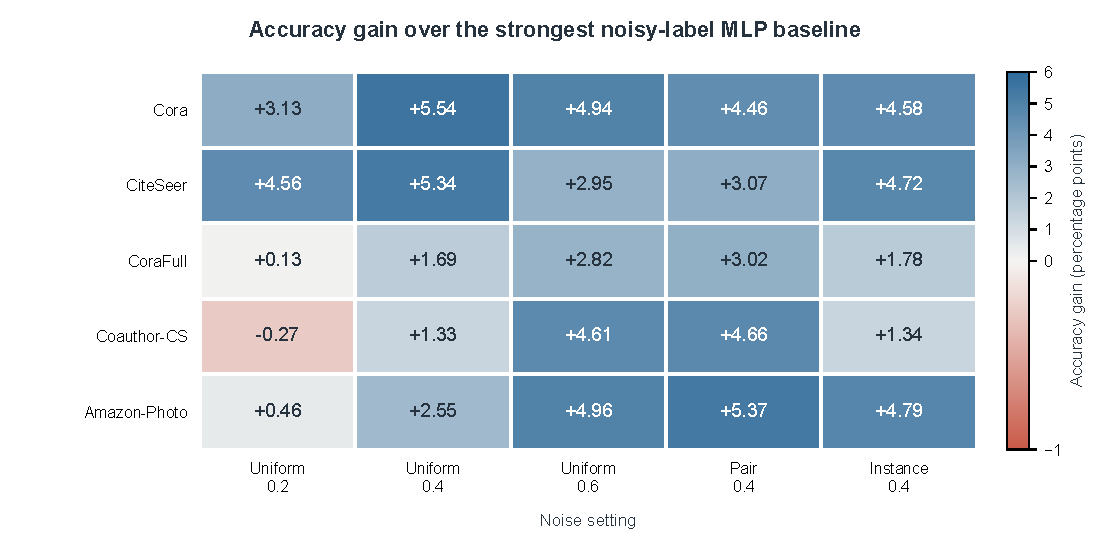
\includegraphics[width=\linewidth]{fig2.pdf}
\caption{Accuracy gain of GB-LCSS over the strongest noisy-label baseline with the same deployed MLP. Each cell shows, in percentage points, the five-seed mean accuracy of GB-LCSS minus the highest mean among the seven baselines for the same dataset and noise setting. Blue and red denote positive and negative gains, respectively.}\label{fig:2}
\end{figure}

Fig.~\ref{fig:3} shows accuracy as a function of the uniform noise rate. As the rate increases from 0.2 to 0.6, GB-LCSS loses less accuracy than MLP+CE and JoCoR on all datasets except CiteSeer.

\begin{figure}
\centering
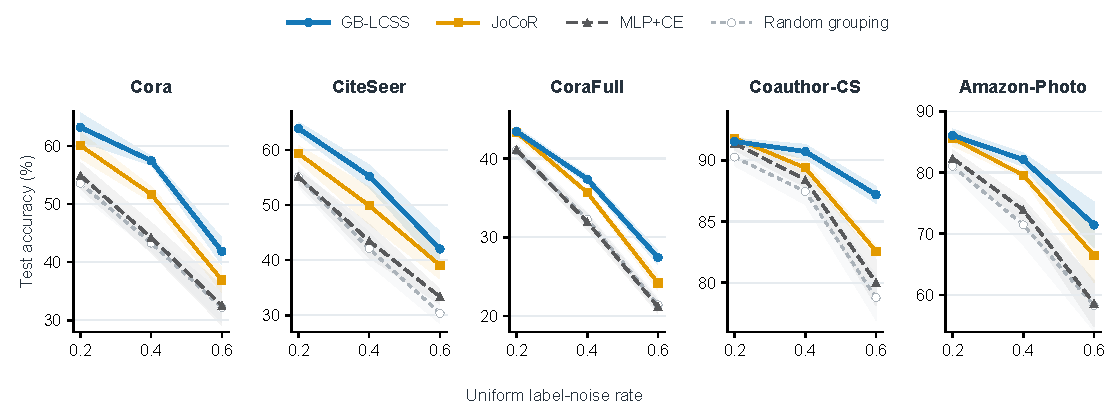
\includegraphics[width=\linewidth]{fig3.pdf}
\caption{Test accuracy under uniform label noise. Lines show the means over five paired seeds, and shaded regions show the sample standard deviations. Panels use different y-axis scales. ``Random grouping'' denotes random size-matched grouping, which preserves the number and sizes of the granular balls.}\label{fig:3}
\end{figure}

On six additional datasets under uniform 0.4 noise, GB-LCSS exceeds random size-matched grouping on all six and the strongest noisy-label baseline on three (Appendix~G).

\subsubsection{Comparison with graph-assisted MLP methods}\label{sec:4.2.2}

Table~\ref{tab:3} compares the graph-assisted MLP methods, which use the graph either to construct soft targets or to shape the representation of the MLP.

\begin{table}
\centering
\caption{Test accuracy of methods that use the graph during MLP training, under uniform 0.4 noise.}\label{tab:3}
\begingroup
\fontsize{9}{11}\selectfont
\setlength{\tabcolsep}{3pt}
\renewcommand{\arraystretch}{1.18}
\setlength{\TableWidth}{\dimexpr\linewidth-12\tabcolsep\relax}
\begin{tabular}{@{}>{\raggedright\arraybackslash}p{\dimexpr 0.140000\TableWidth\relax}>{\raggedright\arraybackslash}p{\dimexpr 0.235000\TableWidth\relax}>{\centering\arraybackslash}p{\dimexpr 0.125000\TableWidth\relax}>{\centering\arraybackslash}p{\dimexpr 0.125000\TableWidth\relax}>{\centering\arraybackslash}p{\dimexpr 0.125000\TableWidth\relax}>{\centering\arraybackslash}p{\dimexpr 0.125000\TableWidth\relax}>{\centering\arraybackslash}p{\dimexpr 0.125000\TableWidth\relax}@{}}
\toprule
\textbf{Method} & \textbf{Use of graph structure in training} & \textbf{Cora} & \textbf{CiteSeer} & \textbf{CoraFull} & \textbf{Coauthor-CS} & \textbf{Amazon-Photo} \\
\midrule
PosteL & Posterior soft labels & 47.09\ensuremath{\pm}1.81 & 45.84\ensuremath{\pm}2.48 & 36.51\ensuremath{\pm}1.01 & 84.74\ensuremath{\pm}1.51 & \underline{80.59\ensuremath{\pm}0.94} \\
ALS & Neighborhood label smoothing & 45.20\ensuremath{\pm}1.24 & 43.77\ensuremath{\pm}2.76 & 31.91\ensuremath{\pm}1.05 & 88.55\ensuremath{\pm}0.86 & 73.41\ensuremath{\pm}2.75 \\
SALS & Structure-aware label smoothing & 48.27\ensuremath{\pm}2.50 & 47.20\ensuremath{\pm}1.69 & \underline{37.06\ensuremath{\pm}0.78} & 88.85\ensuremath{\pm}0.82 & 77.86\ensuremath{\pm}0.79 \\
Graph-MLP & Multi-hop neighborhood-contrastive objective & \textbf{63.23\ensuremath{\pm}3.07} & \textbf{57.23\ensuremath{\pm}1.85} & 37.05\ensuremath{\pm}0.91 & \underline{88.95\ensuremath{\pm}0.43} & 77.05\ensuremath{\pm}1.24 \\
GSDN & Neighborhood self-distillation & 55.97\ensuremath{\pm}4.29 & 50.36\ensuremath{\pm}3.39 & 35.80\ensuremath{\pm}0.66 & 86.55\ensuremath{\pm}0.78 & 73.31\ensuremath{\pm}2.00 \\
GB-LCSS & Label consensus within granular balls & \underline{57.49\ensuremath{\pm}0.76} & \underline{55.24\ensuremath{\pm}2.04} & \textbf{37.39\ensuremath{\pm}0.51} & \textbf{90.71\ensuremath{\pm}0.59} & \textbf{82.12\ensuremath{\pm}1.08} \\
\bottomrule
\end{tabular}
\endgroup
\end{table}


Across the 25 settings, the average accuracy gains over PosteL, ALS, and SALS are 5.69, 7.71, and 4.69 percentage points, respectively. GB-LCSS achieves higher mean accuracy than PosteL and SALS in 24 settings each, and than ALS in all 25 settings (Appendix~E). These methods use graph-defined neighborhoods for target construction, whereas GB-LCSS uses regions of a label-free representation and leave-one-out voting.

Graph-MLP and GSDN use the graph to shape the representation of the MLP and leave the labels unchanged. Under uniform 0.4, GB-LCSS has a higher mean than Graph-MLP on CoraFull, Coauthor-CS, and Amazon-Photo, by 0.34, 1.76, and 5.07 points, respectively, whereas Graph-MLP has the higher mean on Cora and CiteSeer, by 5.74 and 1.99 points. GB-LCSS exceeds GSDN on all five datasets. Graph-MLP and GB-LCSS thus use the training graph in different ways, shaping the learned representation and refining the supervision targets, respectively, and neither is uniformly better across datasets.

\subsection{Ablation and mechanism analysis}\label{sec:4.3}

\subsubsection{Effect of local-consensus targets}\label{sec:4.3.1}

We first examine how the choice of nodes within each ball affects the benefit of local-consensus supervision. Random size-matched grouping shuffles node membership while preserving the ball sizes, and it leaves the target rule unchanged. Uniform and prior smoothing use a fixed coefficient of 0.1 to mix each observed one-hot label with a uniform class distribution or the observed training-label frequencies, respectively. These controls test whether ordinary label smoothing provides similar gains. A further variant includes the current node's own label in the vote under the same tie-handling rule. Table~\ref{tab:4} reports these comparisons under uniform 0.4.

\begin{table}
\centering
\caption{Target-construction ablations under uniform 0.4 noise.}\label{tab:4}
\begingroup
\fontsize{9}{11}\selectfont
\setlength{\tabcolsep}{3pt}
\renewcommand{\arraystretch}{1.18}
\setlength{\TableWidth}{\dimexpr\linewidth-12\tabcolsep\relax}
\begin{tabular}{@{}>{\raggedright\arraybackslash}p{\dimexpr 0.160000\TableWidth\relax}>{\centering\arraybackslash}p{\dimexpr 0.140000\TableWidth\relax}>{\centering\arraybackslash}p{\dimexpr 0.140000\TableWidth\relax}>{\centering\arraybackslash}p{\dimexpr 0.150000\TableWidth\relax}>{\centering\arraybackslash}p{\dimexpr 0.140000\TableWidth\relax}>{\centering\arraybackslash}p{\dimexpr 0.140000\TableWidth\relax}>{\centering\arraybackslash}p{\dimexpr 0.130000\TableWidth\relax}@{}}
\toprule
\textbf{Dataset} & \textbf{GB-LCSS} & \textbf{Own vote included} & \textbf{Random size-matched grouping} & \textbf{Uniform smoothing} & \textbf{Prior smoothing} & \textbf{Gain from\newline excluding\newline own vote} \\
\midrule
Cora & \textbf{57.49\ensuremath{\pm}0.76} & 56.28\ensuremath{\pm}1.54 & 43.31\ensuremath{\pm}1.40 & 44.69\ensuremath{\pm}2.90 & 44.89\ensuremath{\pm}2.38 & +1.21 \\
CiteSeer & \textbf{55.24\ensuremath{\pm}2.04} & 53.52\ensuremath{\pm}2.71 & 42.08\ensuremath{\pm}2.88 & 43.69\ensuremath{\pm}3.31 & 43.43\ensuremath{\pm}2.99 & +1.72 \\
CoraFull & \textbf{37.39\ensuremath{\pm}0.51} & 37.30\ensuremath{\pm}0.57 & 32.30\ensuremath{\pm}0.85 & 32.59\ensuremath{\pm}1.12 & 32.63\ensuremath{\pm}0.84 & +0.09 \\
Coauthor-CS & \textbf{90.71\ensuremath{\pm}0.59} & 90.62\ensuremath{\pm}0.47 & 87.46\ensuremath{\pm}1.07 & 88.25\ensuremath{\pm}0.80 & 88.04\ensuremath{\pm}0.73 & +0.09 \\
Amazon-Photo & \textbf{82.12\ensuremath{\pm}1.08} & 81.33\ensuremath{\pm}0.70 & 71.45\ensuremath{\pm}3.29 & 74.18\ensuremath{\pm}1.72 & 74.72\ensuremath{\pm}1.44 & +0.79 \\
\bottomrule
\end{tabular}
\endgroup
\end{table}


Random size-matched grouping lowers accuracy in all 25 settings, by 8.69 percentage points on average, to approximately the level of MLP+CE. Uniform and prior smoothing recover little of this gain. These controls support the importance of which nodes contribute to the local consensus, beyond target softening alone. Excluding the current node's vote raises mean accuracy on all five datasets under uniform 0.4, as well as on every dataset when averaged over the five noise settings. With clean training labels, targets change only in balls whose training nodes belong to more than one class. Accuracy differs from that of MLP+CE by \ensuremath{-}1.75 to +2.00 percentage points (Appendix~D).


We then assess the training targets themselves, independently of the classifier. Fig.~\ref{fig:4} reports their multiclass Brier score \cite{ref73}, averaged over the labeled training nodes and computed against the clean training labels, which are used only for evaluation:

\[
\frac{1}{|\mathcal V_L|}\sum_{v_n\in\mathcal V_L}\lVert\mathbf t_n-\mathbf e_{y_n}\rVert_2^2.
\]

The score of the observed labels is computed by replacing \(\mathbf t_n\) with \(\mathbf e_{z_n}\). All 25 points, each averaged over five seeds, lie below the equality line: the GB-LCSS targets reduce the score by 0.06--0.51 relative to the observed one-hot targets, with the largest reductions on Coauthor-CS and Amazon-Photo.

\begin{figure}
\centering
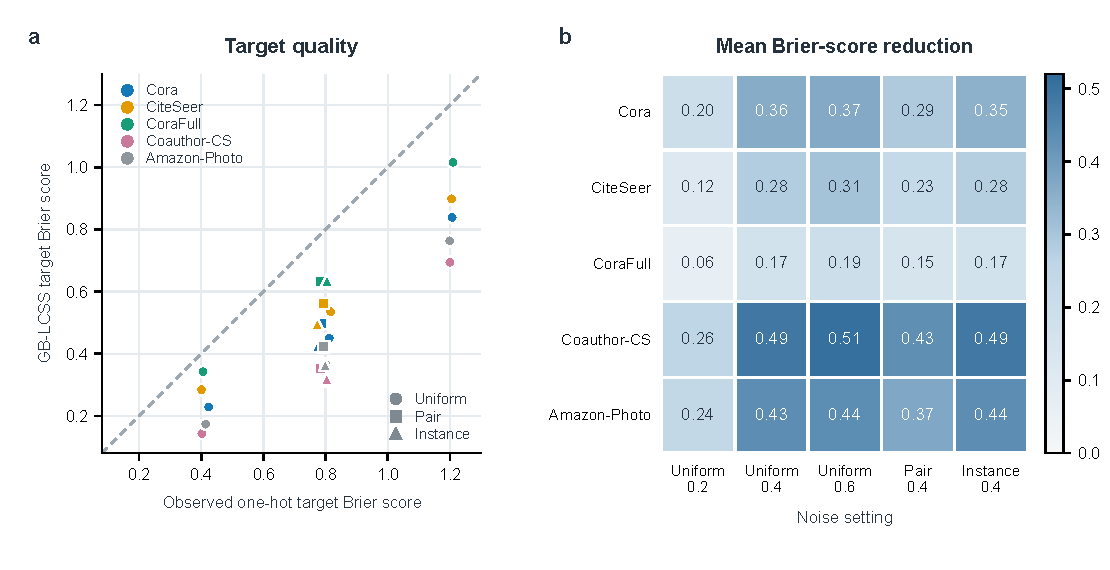
\includegraphics[width=\linewidth]{fig4.pdf}
\caption{Brier scores of the GB-LCSS targets and the observed one-hot targets, computed against the clean training labels. (a) The horizontal and vertical axes show the multiclass Brier scores of the observed one-hot targets and the GB-LCSS targets, respectively. Each marker is the five-seed mean for one dataset--noise setting; colors identify datasets, and circles, squares, and triangles denote uniform, pair, and instance-dependent noise, respectively. The dashed line denotes equality. (b) Each cell shows the observed-target score minus the GB-LCSS target score; positive values indicate a lower squared probability error for the soft targets.}\label{fig:4}
\end{figure}

Using Eq.~(H.5), Appendix~I.2 separates the net Brier-score reduction under uniform 0.4 noise into error removed on corrupted labels and error introduced on correct labels. The reduction exceeds the increase in all 25 dataset--seed runs, by a factor of 6.7--18.1 in the five-seed means.

\subsubsection{Sensitivity to the grouping rule}\label{sec:4.3.2}

This experiment tests whether local-consensus supervision depends on the specific partitioning procedure. We keep the frozen representation and Eqs.~\eqref{eq:7}--\eqref{eq:12} unchanged and replace the granular ball partition with kNN neighborhoods or a k-means partition. For each seed, kNN excludes the query node and matches its neighborhood size to the mean number of training votes per ball; k-means uses the same number of groups as the granular ball partition and likewise excludes the current node's own vote. Table~\ref{tab:5} reports the comparison under uniform 0.4, with differences defined as the accuracy of the alternative grouping minus that of granular ball grouping, in percentage points.

\begin{table}
\centering
\caption{Sensitivity to the grouping rule under uniform 0.4 noise.}\label{tab:5}
\begingroup
\fontsize{9}{11}\selectfont
\setlength{\tabcolsep}{3pt}
\renewcommand{\arraystretch}{1.18}
\setlength{\TableWidth}{\dimexpr\linewidth-10\tabcolsep\relax}
\begin{tabular}{@{}>{\raggedright\arraybackslash}p{\dimexpr 0.190000\TableWidth\relax}>{\centering\arraybackslash}p{\dimexpr 0.170000\TableWidth\relax}>{\centering\arraybackslash}p{\dimexpr 0.160000\TableWidth\relax}>{\centering\arraybackslash}p{\dimexpr 0.140000\TableWidth\relax}>{\centering\arraybackslash}p{\dimexpr 0.170000\TableWidth\relax}>{\centering\arraybackslash}p{\dimexpr 0.170000\TableWidth\relax}@{}}
\toprule
\textbf{Dataset} & \textbf{Granular ball} & \textbf{kNN} & \textbf{kNN \ensuremath{-} GB} & \textbf{k-means} & \textbf{k-means \ensuremath{-} GB} \\
\midrule
Cora & \textbf{57.49\ensuremath{\pm}0.76} & 57.21\ensuremath{\pm}1.19 & \ensuremath{-}0.27 & 56.58\ensuremath{\pm}1.23 & \ensuremath{-}0.91 \\
CiteSeer & 55.24\ensuremath{\pm}2.04 & 56.17\ensuremath{\pm}3.24 & +0.94 & \textbf{56.18\ensuremath{\pm}1.78} & +0.94 \\
CoraFull & 37.39\ensuremath{\pm}0.51 & \textbf{40.50\ensuremath{\pm}0.51} & +3.11 & 39.26\ensuremath{\pm}0.48 & +1.87 \\
Coauthor-CS & 90.71\ensuremath{\pm}0.59 & 90.83\ensuremath{\pm}0.57 & +0.12 & \textbf{91.01\ensuremath{\pm}0.64} & +0.29 \\
Amazon-Photo & 82.12\ensuremath{\pm}1.08 & \textbf{82.23\ensuremath{\pm}1.20} & +0.11 & 81.68\ensuremath{\pm}0.66 & \ensuremath{-}0.44 \\
\bottomrule
\end{tabular}
\par\smallskip\noindent\begin{minipage}{\linewidth}\footnotesize GB denotes granular ball grouping. Differences are in percentage points.\end{minipage}
\endgroup
\end{table}


The three grouping rules yield mean accuracies within one percentage point of one another on four of the five datasets (Table~\ref{tab:5}). All three exceed random size-matched grouping (Tables~\ref{tab:4} and~\ref{tab:5}). These results show that local-consensus targets can also be constructed with other grouping rules. We use granular balls because geometric splitting adapts the partition under explicit size and ball-count constraints, while each ball provides shared class counts for constructing its members' targets. Section~\ref{sec:4.4.2} examines the construction time and storage requirements of this design.

\subsubsection{Effect of the representation space}\label{sec:4.3.3}

To examine how the representation affects grouping and target construction, Table~\ref{tab:6} compares GRACE, raw node attributes \(\mathbf{X}\), and two-step propagated attributes \(\mathbf{A}^2\mathbf{X}\) on the five datasets under uniform 0.4 noise, using five paired seeds, fixed splitting parameters, and the main training protocol. Ball counts are reported as ranges across these seeds. For \(\mathbf{A}^2\mathbf{X}\), the attributes are multiplied twice by the original adjacency matrix, without added self-loops or normalization, and the resulting vectors are normalized as in Eq.~\eqref{eq:3}.

\begin{table}
\centering
\caption{Effect of the representation used for partitioning under uniform 0.4 noise.}\label{tab:6}
\begingroup
\fontsize{9}{11}\selectfont
\setlength{\tabcolsep}{5pt}
\renewcommand{\arraystretch}{1.18}
\begin{tabular*}{\linewidth}{@{\extracolsep{\fill}}lcccccc@{}}
\toprule
\textbf{Dataset} & \multicolumn{3}{c}{\textbf{Accuracy}} & \multicolumn{3}{c}{\textbf{Number of balls}}\\
\cmidrule(lr){2-4}\cmidrule(l){5-7}
& GRACE & Raw \(\mathbf{X}\) & \(\mathbf{A}^2\mathbf{X}\) & GRACE & Raw \(\mathbf{X}\) & \(\mathbf{A}^2\mathbf{X}\)\\
\midrule
Cora & \textbf{57.49\ensuremath{\pm}0.76} & 44.37\ensuremath{\pm}2.31 & 44.37\ensuremath{\pm}2.31 & 52--53 & 1 & 1 \\
CiteSeer & \textbf{55.24\ensuremath{\pm}2.04} & 42.90\ensuremath{\pm}2.50 & 42.90\ensuremath{\pm}2.50 & 63--64 & 1 & 1 \\
CoraFull & \textbf{37.39\ensuremath{\pm}0.51} & 31.86\ensuremath{\pm}1.05 & 31.86\ensuremath{\pm}1.05 & 64 & 1 & 1 \\
Coauthor-CS & \textbf{90.71\ensuremath{\pm}0.59} & 87.63\ensuremath{\pm}1.10 & 89.20\ensuremath{\pm}0.67 & 64 & 1 & 50--59 \\
Amazon-Photo & \textbf{82.12\ensuremath{\pm}1.08} & 73.37\ensuremath{\pm}1.13 & 81.13\ensuremath{\pm}1.64 & 64 & 1 & 64 \\
\bottomrule
\end{tabular*}
\endgroup
\end{table}


With raw \(\mathbf{X}\), no split satisfies Eq.~\eqref{eq:6} in any of the 25 dataset--seed runs, so all nodes remain in one ball and each node draws its consensus from all other training nodes. The \(\mathbf{A}^2\mathbf{X}\) representation likewise produces a single ball on Cora, CiteSeer, and CoraFull. It produces 50--59 and 64 balls on Coauthor-CS and Amazon-Photo, respectively, where its accuracy exceeds that of raw \(\mathbf{X}\). GRACE yields a multi-ball partition on every dataset and the highest mean accuracy among the three representations, exceeding \(\mathbf{A}^2\mathbf{X}\) by 1.51 points on Coauthor-CS and 0.99 points on Amazon-Photo. 

On Cora, CiteSeer, and CoraFull, we train three GRACE representations with different pretraining seeds and evaluate each representation using three downstream seeds. Partitions obtained from different pretraining seeds differ substantially, with adjusted Rand indices \cite{ref74} between 0.247 and 0.365. After averaging over downstream seeds, the standard deviations of accuracy across pretraining seeds are 0.13, 0.45, and 0.60 percentage points, respectively, and GB-LCSS exceeds MLP+CE for every pretraining seed. Thus, although the node assignments change substantially across pretraining seeds, downstream accuracy changes little.

\subsubsection{Sensitivity to construction and target parameters}\label{sec:4.3.4}

Appendix~I.1 varies one grouping or voting parameter at a time on the five datasets under uniform 0.4 noise, with fixed representations and five paired seeds. The largest losses occur when a higher splitting threshold leaves all nodes in one ball or when a higher voting threshold sharply reduces the number of nodes receiving consensus supervision. The remaining tested settings stay within three percentage points of the default. A larger ball budget improves accuracy on CoraFull, and assigning more weight to the most-voted class improves accuracy on four datasets.

\subsection{Graph-teacher extension and computational cost}\label{sec:4.4}

\subsubsection{Graph-teacher distillation}\label{sec:4.4.1}

We next examine whether training a graph teacher with GB-LCSS targets also improves its distilled MLP student (\hyperref[sec:3.5]{Section~\ref*{sec:3.5}}). Table~\ref{tab:7} compares direct MLP training with five distillation routes on the five datasets under uniform 0.4 and 0.6. The first row trains the MLP on the labeled nodes only, whereas the remaining rows use teacher predictions with method-specific objectives and node selection; all routes deploy the same two-layer MLP. The GCN teacher trained on GB-LCSS targets differs from the GCN(X)+CE baseline only in using the soft target of Eq.~\eqref{eq:12} in place of the observed one-hot label; the other routes are described in \hyperref[sec:4.1.3]{Section~\ref*{sec:4.1.3}} and Appendix~F.

\begin{table}
\centering
\caption{Test accuracy of deployed MLPs under direct training and graph-to-MLP distillation.}\label{tab:7}
{\small\textbf{(a) Uniform 0.4}}\par\smallskip

\begingroup
\fontsize{9}{11}\selectfont
\setlength{\tabcolsep}{3pt}
\renewcommand{\arraystretch}{1.18}
\setlength{\TableWidth}{\dimexpr\linewidth-10\tabcolsep\relax}
\begin{tabular}{@{}>{\raggedright\arraybackslash}p{\dimexpr 0.320000\TableWidth\relax}>{\centering\arraybackslash}p{\dimexpr 0.136000\TableWidth\relax}>{\centering\arraybackslash}p{\dimexpr 0.136000\TableWidth\relax}>{\centering\arraybackslash}p{\dimexpr 0.136000\TableWidth\relax}>{\centering\arraybackslash}p{\dimexpr 0.136000\TableWidth\relax}>{\centering\arraybackslash}p{\dimexpr 0.136000\TableWidth\relax}@{}}
\toprule
\textbf{Training route} & \textbf{Cora} & \textbf{CiteSeer} & \textbf{CoraFull} & \textbf{Coauthor-CS} & \textbf{Amazon-Photo} \\
\midrule
GB-LCSS, direct MLP training & 57.49\ensuremath{\pm}0.76 & 55.24\ensuremath{\pm}2.04 & 37.39\ensuremath{\pm}0.51 & 90.71\ensuremath{\pm}0.59 & 82.12\ensuremath{\pm}1.08 \\
\midrule
GCN(X)+CE teacher & 77.95\ensuremath{\pm}2.62 & 66.09\ensuremath{\pm}1.38 & \textbf{58.74\ensuremath{\pm}0.82} & 93.20\ensuremath{\pm}0.09 & 89.86\ensuremath{\pm}0.77 \\
FF-G2M & 77.65\ensuremath{\pm}2.97 & 65.80\ensuremath{\pm}0.49 & 56.58\ensuremath{\pm}0.93 & 91.58\ensuremath{\pm}0.24 & 84.82\ensuremath{\pm}0.84 \\
KRD & 71.77\ensuremath{\pm}2.20 & 64.96\ensuremath{\pm}1.03 & 47.12\ensuremath{\pm}0.95 & 91.39\ensuremath{\pm}0.49 & 85.17\ensuremath{\pm}0.94 \\
VQGraph & 78.89\ensuremath{\pm}2.34 & 65.64\ensuremath{\pm}1.72 & 58.52\ensuremath{\pm}0.77 & 93.25\ensuremath{\pm}0.09 & \textbf{90.54\ensuremath{\pm}0.85} \\
GCN teacher trained on GB-LCSS targets & \textbf{81.35\ensuremath{\pm}1.05} & \textbf{69.27\ensuremath{\pm}1.57} & 57.29\ensuremath{\pm}0.24 & \textbf{93.83\ensuremath{\pm}0.21} & 90.40\ensuremath{\pm}0.77 \\
\bottomrule
\end{tabular}
\endgroup


\par\medskip{\small\textbf{(b) Uniform 0.6}}\par\smallskip

\begingroup
\fontsize{9}{11}\selectfont
\setlength{\tabcolsep}{3pt}
\renewcommand{\arraystretch}{1.18}
\setlength{\TableWidth}{\dimexpr\linewidth-10\tabcolsep\relax}
\begin{tabular}{@{}>{\raggedright\arraybackslash}p{\dimexpr 0.320000\TableWidth\relax}>{\centering\arraybackslash}p{\dimexpr 0.136000\TableWidth\relax}>{\centering\arraybackslash}p{\dimexpr 0.136000\TableWidth\relax}>{\centering\arraybackslash}p{\dimexpr 0.136000\TableWidth\relax}>{\centering\arraybackslash}p{\dimexpr 0.136000\TableWidth\relax}>{\centering\arraybackslash}p{\dimexpr 0.136000\TableWidth\relax}@{}}
\toprule
\textbf{Training route} & \textbf{Cora} & \textbf{CiteSeer} & \textbf{CoraFull} & \textbf{Coauthor-CS} & \textbf{Amazon-Photo} \\
\midrule
GB-LCSS, direct MLP training & 41.86\ensuremath{\pm}2.30 & 42.02\ensuremath{\pm}3.14 & 27.43\ensuremath{\pm}0.89 & 87.19\ensuremath{\pm}0.69 & 71.45\ensuremath{\pm}3.75 \\
\midrule
GCN(X)+CE teacher & 65.50\ensuremath{\pm}3.28 & 53.30\ensuremath{\pm}4.42 & 51.63\ensuremath{\pm}2.02 & 91.13\ensuremath{\pm}0.58 & 84.80\ensuremath{\pm}1.48 \\
FF-G2M & 63.63\ensuremath{\pm}2.16 & 52.32\ensuremath{\pm}4.20 & 45.78\ensuremath{\pm}2.90 & 86.50\ensuremath{\pm}1.01 & 73.08\ensuremath{\pm}2.82 \\
KRD & 61.28\ensuremath{\pm}1.17 & 54.17\ensuremath{\pm}3.14 & 41.61\ensuremath{\pm}2.43 & 89.80\ensuremath{\pm}0.29 & 80.30\ensuremath{\pm}0.51 \\
VQGraph & 65.75\ensuremath{\pm}2.72 & 53.34\ensuremath{\pm}4.47 & 52.01\ensuremath{\pm}0.65 & 90.71\ensuremath{\pm}1.24 & 84.77\ensuremath{\pm}2.19 \\
GCN teacher trained on GB-LCSS targets & \textbf{71.34\ensuremath{\pm}3.91} & \textbf{58.93\ensuremath{\pm}4.62} & \textbf{52.32\ensuremath{\pm}1.26} & \textbf{92.40\ensuremath{\pm}0.65} & \textbf{86.81\ensuremath{\pm}1.94} \\
\bottomrule
\end{tabular}
\endgroup


\end{table}

Training the GCN teacher with GB-LCSS targets instead of the observed labels raises the mean accuracy of the distilled student in nine of the ten settings; the only exception is CoraFull under uniform 0.4. Target refinement can therefore improve the supervision transferred through a graph teacher. Among the five distillation routes, this student attains the highest mean accuracy in eight of the ten settings; on CoraFull and Amazon-Photo under uniform 0.4, GCN(X)+CE and VQGraph are higher by 1.45 and 0.14 points, respectively. The distilled student exceeds direct MLP training in all ten settings, by 3.12--23.86 points under uniform 0.4 and 5.21--29.48 points under uniform 0.6. The extension adds a GCN teacher and distillation over all nodes during training, while retaining the same MLP architecture at inference.
\subsubsection{Computational cost}\label{sec:4.4.2}

GB-LCSS and MLP+CE deploy the same MLP, so we measure the additional training-time costs. Timing and GPU-memory measurements were obtained on a Windows 10 (build 19045) workstation with an AMD Radeon RX 7700 XT GPU, using Python 3.12.10, PyTorch 2.9.1+rocm7.2.1, and PyTorch Geometric 2.7.0. GRACE pretraining takes 0.07, 0.13, and 74.48 minutes on Cora, CiteSeer, and CoraFull, respectively, with peak allocated GPU memory of 0.40, 0.67, and 12.73 GiB. Times are averaged over three pretraining seeds, and memory is the largest peak across these runs reported by \texttt{torch.cuda.max\_memory\_allocated()}. Each frozen representation is computed once per dataset and reused across all noise settings and downstream seeds.

Fig.~\ref{fig:5} compares the construction time and storage of the three grouping rules. The granular ball partition stores one class-count vector per ball, whereas exact kNN stores one neighbor list per training node. In the seed-0 measurements, granular ball grouping requires less storage than exact kNN on CoraFull, Coauthor-CS, and Amazon-Photo, with the largest differences on the two largest graphs. Its construction time is also the shortest among the three grouping rules on three of the five datasets.

\begin{figure}
\centering
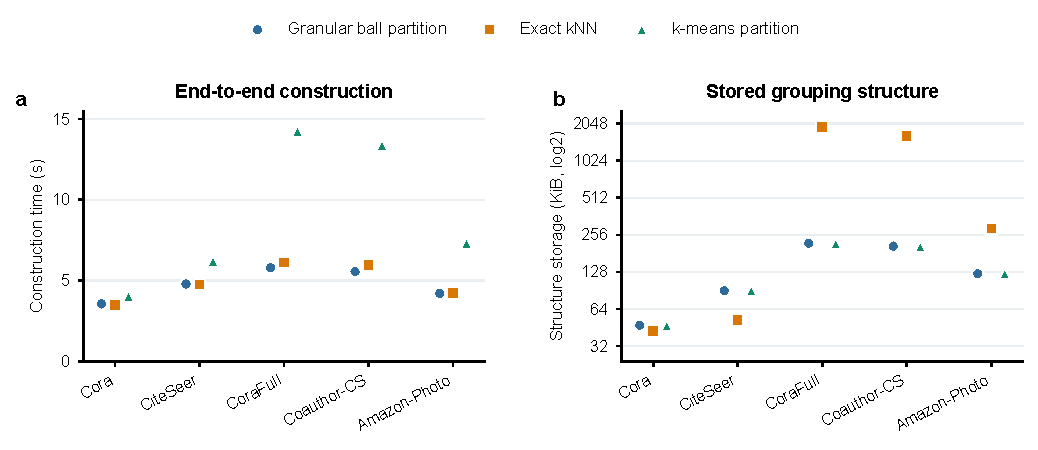
\includegraphics[width=\linewidth]{fig5.pdf}
\caption{Construction cost of granular ball, exact-kNN, and k-means grouping. (a) End-to-end construction time. (b) Storage of the grouping structure. Both panels show seed-0 measurements.}\label{fig:5}
\end{figure}

\subsection{Discussion}\label{sec:4.5}

When the other training labels in a ball provide consistent evidence for the underlying class, their consensus can offset an isolated annotation error. The label-free representation determines which nodes contribute this evidence, and the random-grouping and label-smoothing controls support the importance of this choice beyond target softening alone (Table~\ref{tab:4}). Leave-one-out voting keeps the current annotation out of its own consensus estimate, a property used in the conditional expected-error analysis of Corollary~\ref{cor:expected}. Under uniform 0.4 noise, the reduction in Brier error on corrupted labels exceeds the error introduced on correctly labeled nodes (Appendix~I.2).

The usefulness of local evidence depends on both its class composition and the number of available votes. Proposition~\ref{prop:local_vote} relates these quantities to voting reliability under independent symmetric noise. Agreement alone is insufficient when the local labels favor an incorrect class, since the consensus can then move the target away from the true class. The representation and parameter studies show lower accuracy when local groups fail to form or voting support becomes sparse. Under uniform 0.4 noise, CoraFull has both the lowest proportion of training nodes with a positive clean-vote margin (36.13\%) and the smallest net reduction in target Brier score among the five datasets (Appendix~I.2). With clean training labels, refinement raises mean accuracy on one dataset and lowers it on four, with all changes within 2.00 percentage points (Appendix~D). On the six additional datasets, GB-LCSS exceeds the strongest noisy-label baseline on three (Appendix~G). These results indicate that the benefit varies across datasets and supervision conditions.

GB-LCSS, Graph-MLP, and GLNN share an attribute-only deployment interface but use the training graph differently. Graph-MLP shapes the representation through a neighborhood-contrastive objective, GLNN transfers predictions from a GNN teacher, and GB-LCSS refines supervision targets. GB-LCSS and Graph-MLP have dataset-dependent advantages (Table~\ref{tab:3}). The distillation experiment shows that training the same GCN teacher with GB-LCSS targets can also benefit its MLP student (Table~\ref{tab:7}). These targets can therefore support both direct MLP training and graph-to-MLP distillation.

Granular balls provide a practical organization for local-consensus supervision. Each node belongs to one ball, whose class counts are shared when constructing targets for its training nodes. Geometric splitting adapts the partition to the representation while limiting the number of balls and enforcing a minimum size for each child ball. Granular ball grouping requires less storage than exact kNN on the three larger graphs and has the shortest construction time on three datasets (Fig.~\ref{fig:5}). These results support its use as a grouping mechanism that combines competitive accuracy, shared regional statistics, and controlled construction costs.

\section{Conclusion}\label{sec:5}

We presented GB-LCSS for learning from noisy training labels when the deployed classifier receives only node attributes. The method organizes nodes into granular balls in a frozen, label-free graph representation and combines each observed label with the consensus of the other training nodes in its ball. Our analysis relates local-vote reliability to the number of available votes and their clean-class margin under symmetric noise, decomposes the squared error of the soft target, and gives a sufficient condition for it to have lower expected error than the observed label.

Across five datasets and five noise settings, GB-LCSS achieves the highest five-seed mean accuracy in 24 of the 25 settings, compared with seven noisy-label baselines that use the same deployed MLP architecture. Its soft targets have lower mean Brier scores than the observed one-hot labels in all 25 settings. The controlled comparisons support the importance of which training nodes contribute to the local consensus, with granular balls providing a compact way to share label statistics. The distillation experiments further show that these targets can improve the MLP student when they are used to train its graph teacher.

The present evaluation focuses on synthetic label noise in a fixed-graph transductive setting, with clean validation labels used for model selection. Future work will test the method on naturally occurring annotation errors and develop model-selection procedures for imperfect validation labels. Another direction is to evaluate generalization to newly arriving nodes and to investigate how the representations and granular ball partitions can be updated as the training graph grows.
\section*{Acknowledgements}

This work was supported by the Yangtze River Delta Social Assistance Public Service Platform (B801065001FY050) and the National Natural Science Foundation of China (Nos. 62276136, 62206129, and 62375133).

\setlength{\bibsep}{0.5pt plus 0.2pt minus 0.2pt}

\bibliographystyle{cas-model2-names}
\bibliography{references}
\end{document}
